\section{Results}

\subsection{PyTorch Bugs} \label{results:pytorch-bugs}

Based on the findings during this project we've applied to talk at the Positive Hack Days (PHD) 2023 conference. The talk was accepted, and we presented our findings at the conference.

\subsubsection{\#91999: Case study of a bug in PyTorch}
\subsubsection{\#91999: Case study of a bug in PyTorch}

\subsection{Experimental Results for the Scheduling Strategy} \label{results:symbolic-pointers-modeling-scheduling}

To assess the quality of proposed changes we have conducted multiple experiments.

The first one: symptr-15-1

\begin{figure}[h]
    \centering
    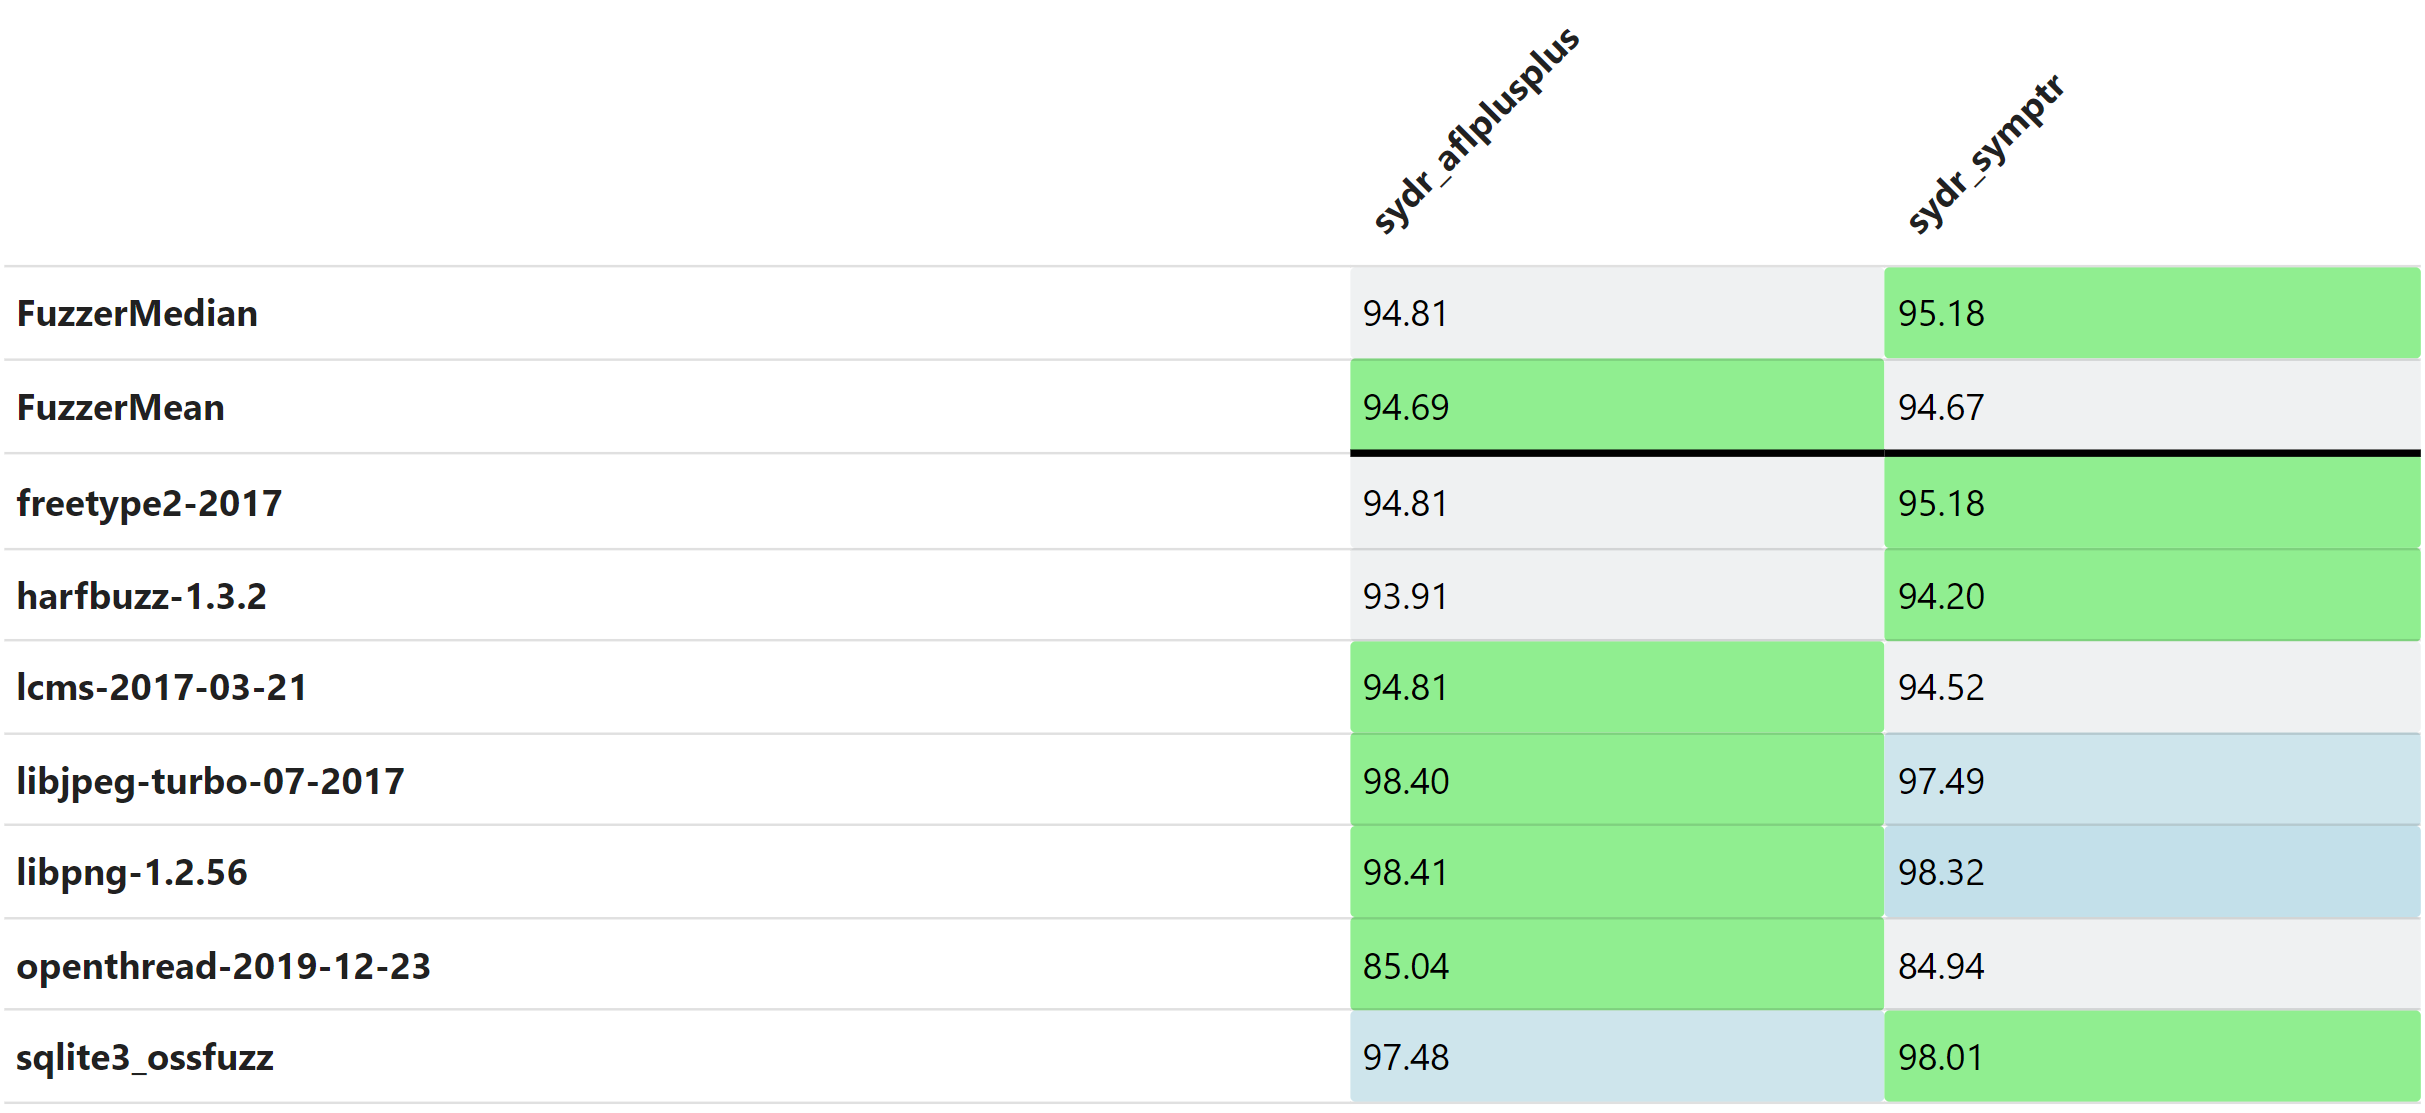
\includegraphics[width=0.9\textwidth]{assets/fuzzbench/symptr-15-1/median-relative-code-coverage-on-each-benchmark.png}
    \caption{Median relative code coverage on each benchmark (N=15)}
    \label{fig:fuzzbench-symptr-15-1-coverage}
\end{figure}

\begin{figure}[h]
    \centering
    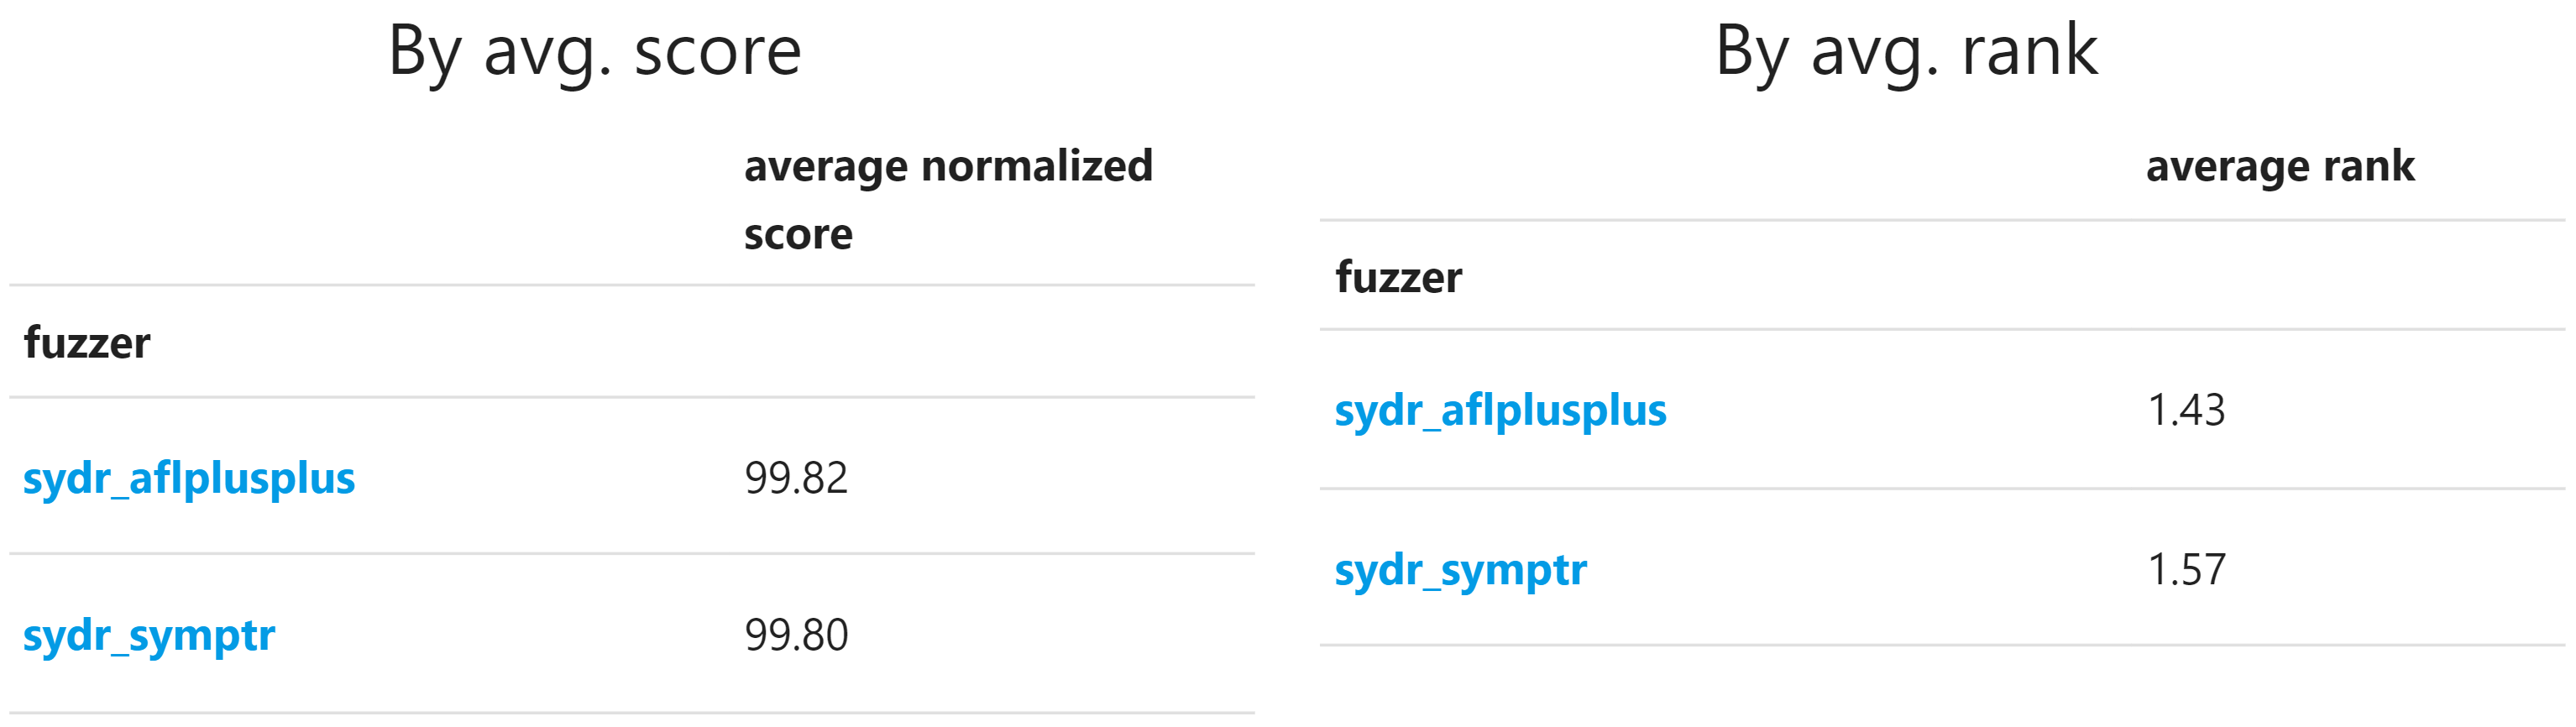
\includegraphics[width=0.9\textwidth]{assets/fuzzbench/symptr-15-1/avg-score-avg-rank.png}
    \caption{Average score and average rank (N=15)}
    \label{fig:fuzzbench-symptr-15-1-score-rank}
\end{figure}

The second one: symptr-25-1

\begin{figure}[h]
    \centering
    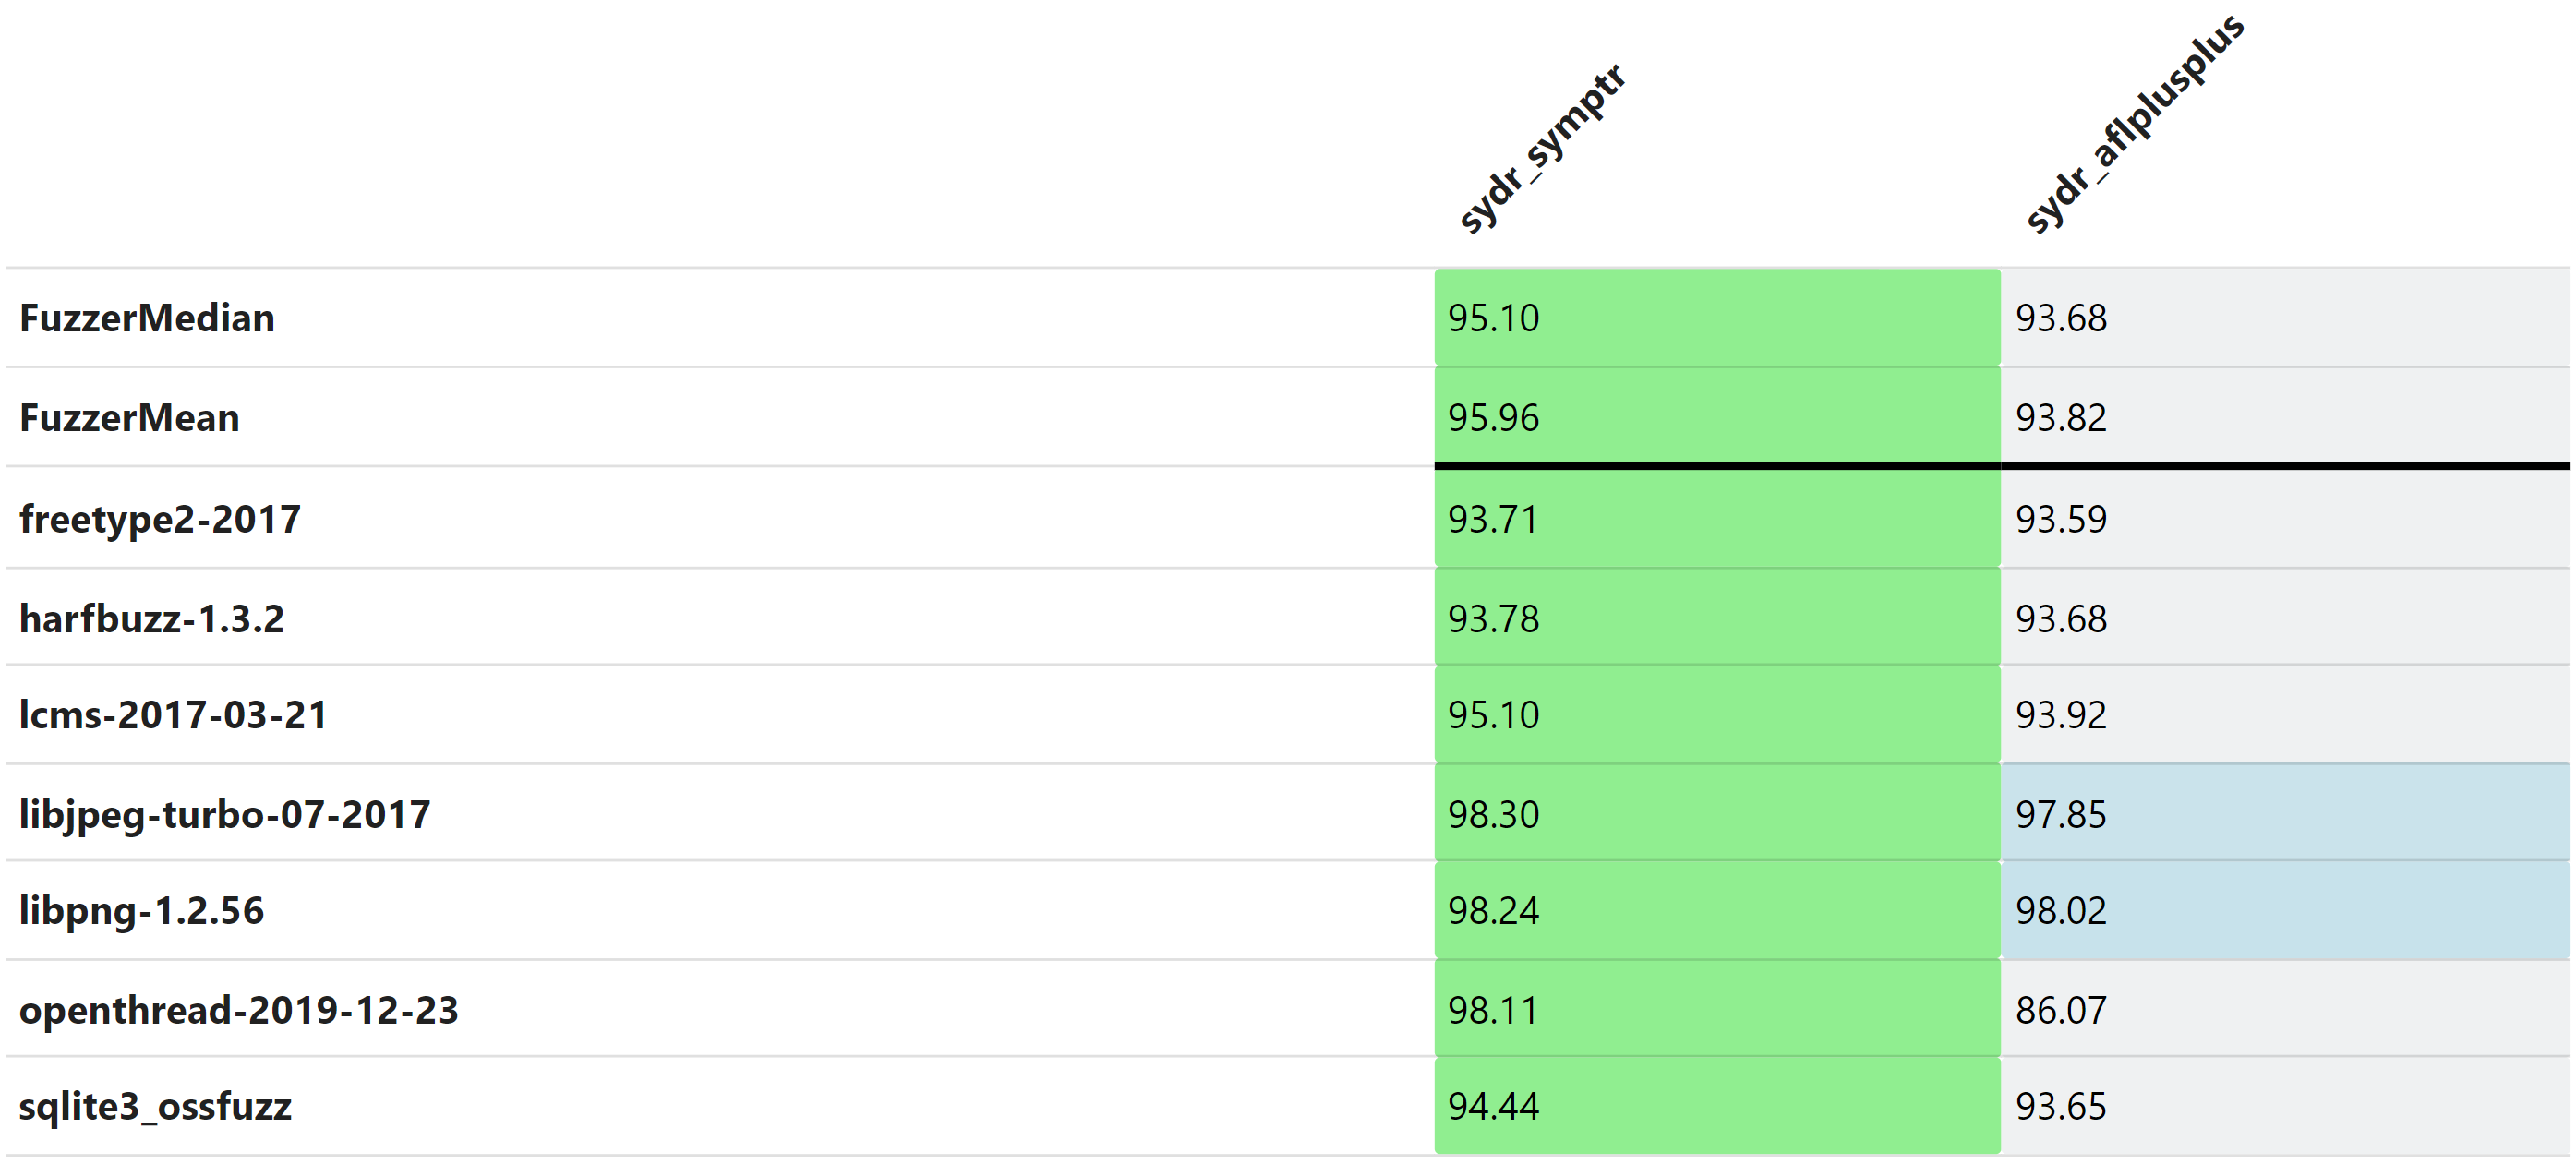
\includegraphics[width=0.9\textwidth]{assets/fuzzbench/symptr-25-1/median-relative-code-coverage-on-each-benchmark.png}
    \caption{Median relative code coverage on each benchmark (N=25)}
    \label{fig:fuzzbench-symptr-25-1-coverage}
\end{figure}

\begin{figure}[h]
    \centering
    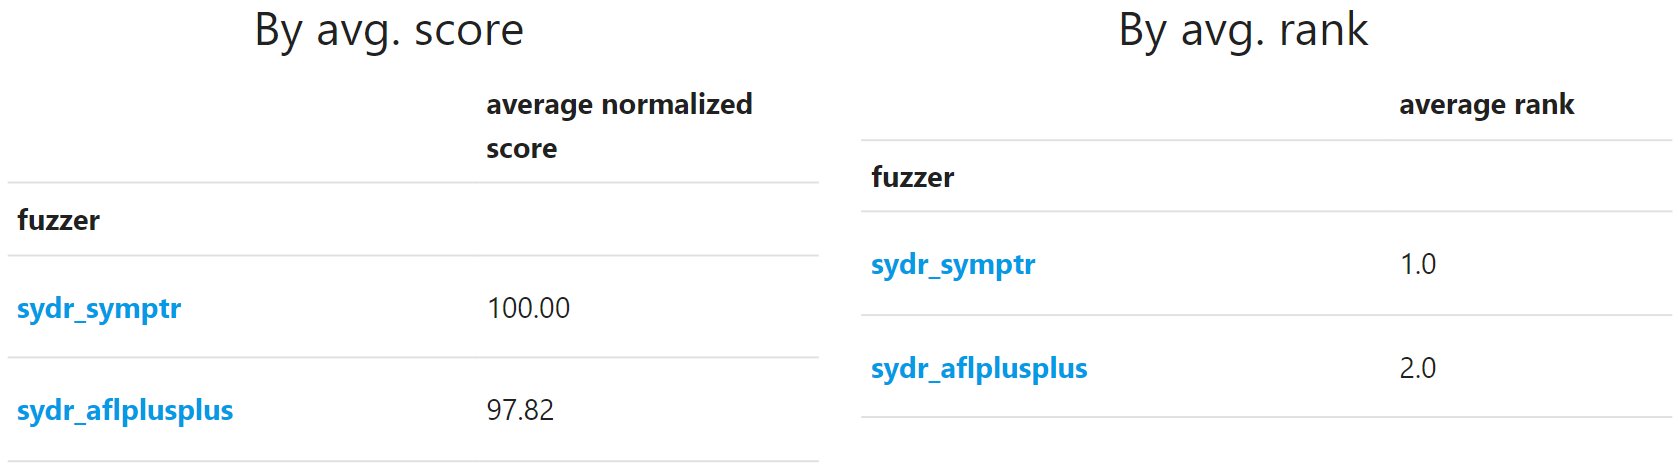
\includegraphics[width=0.9\textwidth]{assets/fuzzbench/symptr-25-1/avg-score-avg-rank.png}
    \caption{Average score and average rank (N=25)}
    \label{fig:fuzzbench-symptr-25-1-score-rank}
\end{figure}

\newpage

And, finally, the third one: symptr-25-vs-35-2

\begin{figure}[h]
    \centering
    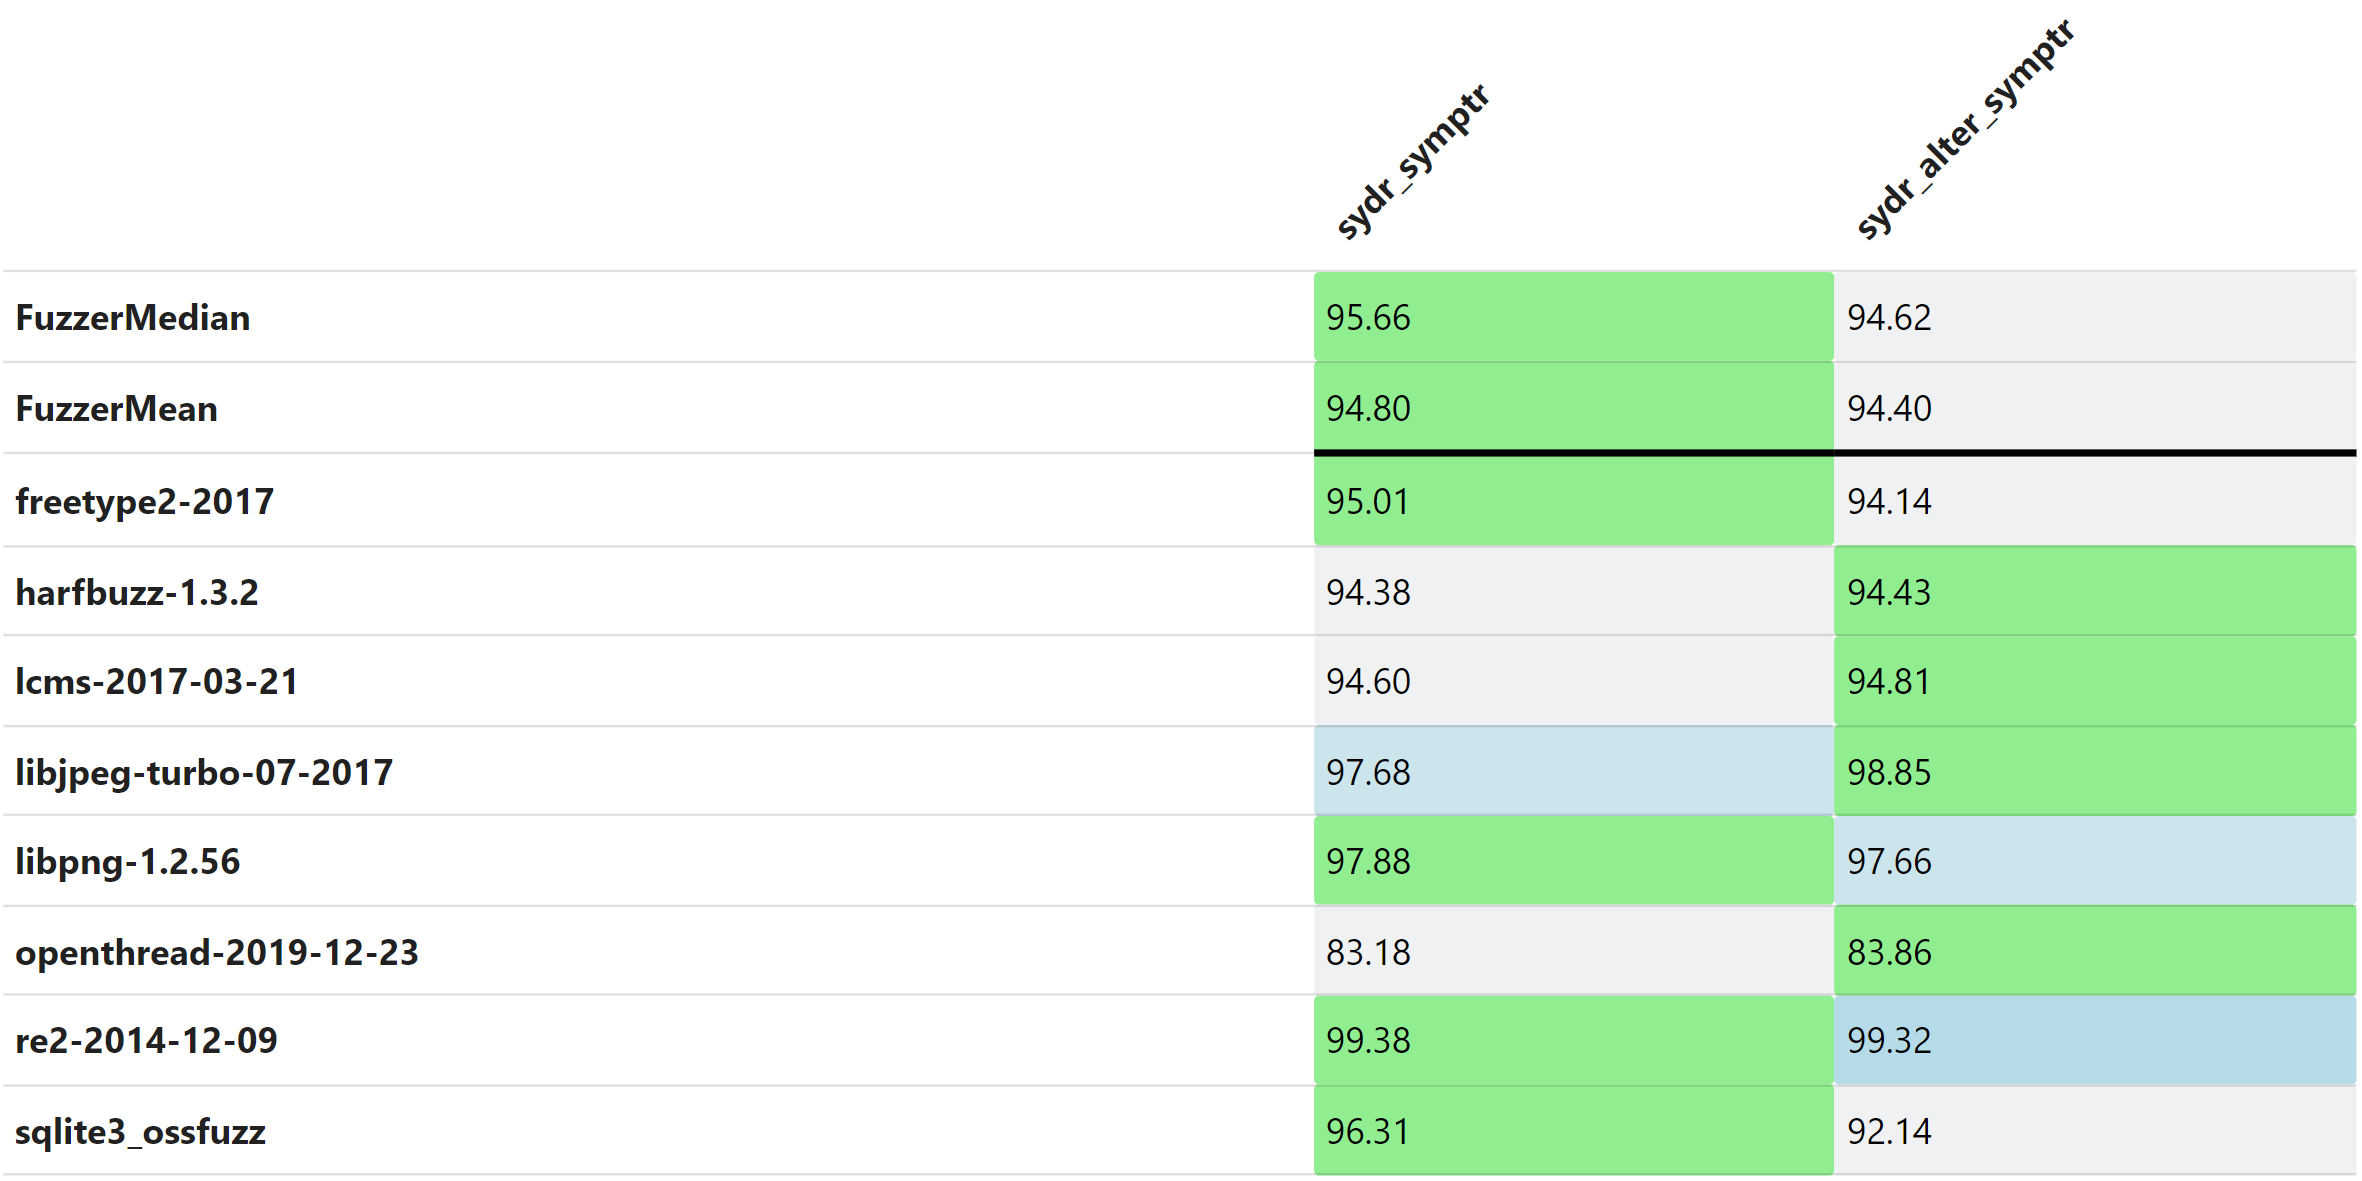
\includegraphics[width=0.9\textwidth]{assets/fuzzbench/symptr-25-vs-35-2/median-relative-code-coverage-on-each-benchmark.png}
    \caption{Median relative code coverage on each benchmark (N=25 vs N=35)}
    \label{fig:fuzzbench-symptr-25-vs-35-2-coverage}
\end{figure}

\begin{figure}[h]
    \centering
    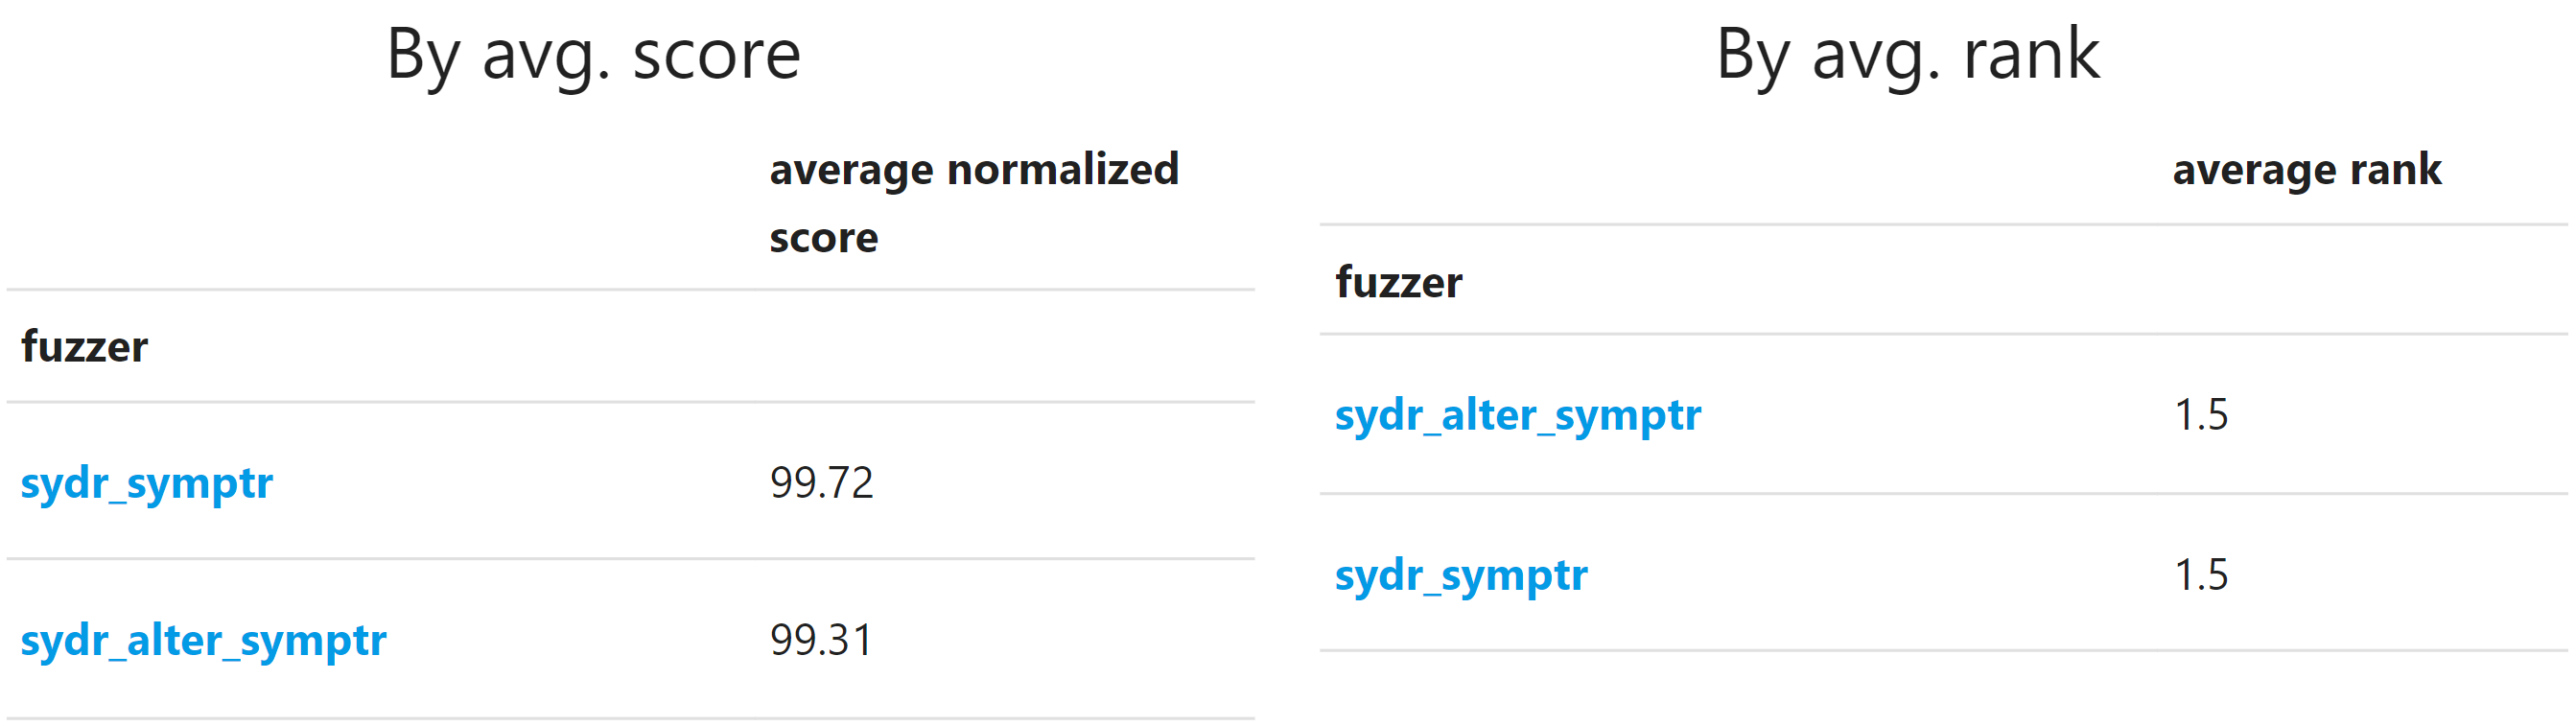
\includegraphics[width=0.9\textwidth]{assets/fuzzbench/symptr-25-vs-35-2/avg-score-avg-rank.png}
    \caption{Average score and average rank (N=25 vs N=35)}
    \label{fig:fuzzbench-symptr-25-vs-35-2-score-rank}
\end{figure}

\subsection{Annotate} \label{results:annotate}

\definecolor{Gray}{gray}{0.9}
\newcolumntype{g}{>{\columncolor{Gray}}c}
\begin{table}[h]
    \centering
    \begin{tabular}{cgcgcg}
        \toprule
        \multirow{2}{*}{\bfseries Benchmark} & \multicolumn{2}{c}{\bfseries Default (ms)} & \multicolumn{2}{c}{\bfseries Rust (ms)} & \textbf{Performance diff}                            \\
                                             & Mean                                       & Std                                     & Mean                      & Std          &           \\
        cjson                                & 292.25                                     & $ \pm 66.1337 $                         & 1.08                      & $ \pm 0.06 $ & -99.63 \% \\
        libjpeg                              & 931.96                                     & $ \pm 55.3113 $                         & 1.75                      & $ \pm 0.19 $ & -99.81 \% \\
        libpng                               & 924.03                                     & $ \pm 567.277 $                         & 1.64                      & $ \pm 0.26 $ & -99.82 \% \\
        libxml2                              & 38308.54                                   & $ \pm 796.162 $                         & 12.27                     & $ \pm 0.33 $ & -99.97 \% \\
        minigzip                             & 14567.67                                   & $ \pm 121.165 $                         & 7.51                      & $ \pm 0.48 $ & -99.94 \% \\
        pcre2                                & 14562.59                                   & $ \pm 1419.99 $                         & 7.26                      & $ \pm 0.58 $ & -99.95 \% \\
        readelf                              & 19486.86                                   & $ \pm 1015.72 $                         & 7.02                      & $ \pm 0.36 $ & -99.96 \% \\
        rizin                                & 31061.09                                   & $ \pm 1800.72 $                         & 12.77                     & $ \pm 0.22 $ & -99.96 \% \\
        yices                                & 8936.02                                    & $ \pm 111.98 $                          & 3.98                      & $ \pm 0.3 $  & -99.96 \% \\
        yodl                                 & 16907.58                                   & $ \pm 377.37 $                          & 7.97                      & $ \pm 0.31 $ & -99.95 \% \\
        \bottomrule
    \end{tabular}
    \caption{Mean execution time to annotate 10 branch traces with the default and Rust annotator.}
    \label{table:annotate-branch-traces-10}
\end{table}

\definecolor{Gray}{gray}{0.9}
\newcolumntype{g}{>{\columncolor{Gray}}c}
\begin{table}[h]
    \centering
    \resizebox{\columnwidth}{!}{%
        \begin{tabular}{ccgcgcg}
            \toprule
            \multirow{2}{*}{\bfseries Benchmark} & \multirow{2}{*}{\bfseries Size (mb)} & \multicolumn{2}{c}{\bfseries Default (s)} & \multicolumn{2}{c}{\bfseries Rust (s)} & \textbf{Performance diff}                             \\
                                                 &                                      & Mean                                      & Std                                    & Mean                      & Std           &           \\
            cjson                                & 1.21                                 & 20.74                                     & $ \pm 0.05 $                           & 0.23                      & $ \pm 0.005 $ & -98.87 \% \\
            libjpeg                              & 6.69                                 & 176.9                                     & $ \pm 0.60 $                           & 2.32                      & $ \pm 0.027 $ & -98.69 \% \\
            libpng                               & 2.08                                 & 57.6                                      & $ \pm 0.36 $                           & 0.75                      & $ \pm 0.019 $ & -98.69 \% \\
            libxml2                              & 50.3                                 & timeout                                   & timeout                                & 21.27                     & $ \pm 1.016 $ & XXX \%    \\
            minigzip                             & 0.75                                 & timeout                                   & timeout                                & 166.59                    & $ \pm 1.863 $ & XXX \%    \\
            pcre2                                & 6.62                                 & 172.77                                    & $ \pm 0.69 $                           & 2.8                       & $ \pm 0.048 $ & -98.38 \% \\
            readelf                              & 9.19                                 & 454.11                                    & $ \pm 40.68 $                          & 3.94                      & $ \pm 0.144 $ & -99.13 \% \\
            rizin                                & 34.04                                & timeout                                   & timeout                                & 15.15                     & $ \pm 0.925 $ & XXX \%    \\
            yices                                & 10.48                                & 294                                       & $ \pm 1.1 $                            & 4.69                      & $ \pm 0.123 $ & -98.4 \%  \\
            yodl                                 & 22.53                                & timeout                                   & timeout                                & 10.3                      & $ \pm 1.014 $ & XXX \%    \\
            \bottomrule
        \end{tabular}
    }
    \caption{Mean execution time (over 3 runs) to annotate instruction trace with the default and Rust annotator.}
    \label{table:annotate-instruction-trace-3}
\end{table}